\section{Results}
\label{sec:results}

\subsection{Eight passes: verdicts against labels, and against the vendors' own recipes}
\label{sec:eight}

\begin{figure}[t]\centering
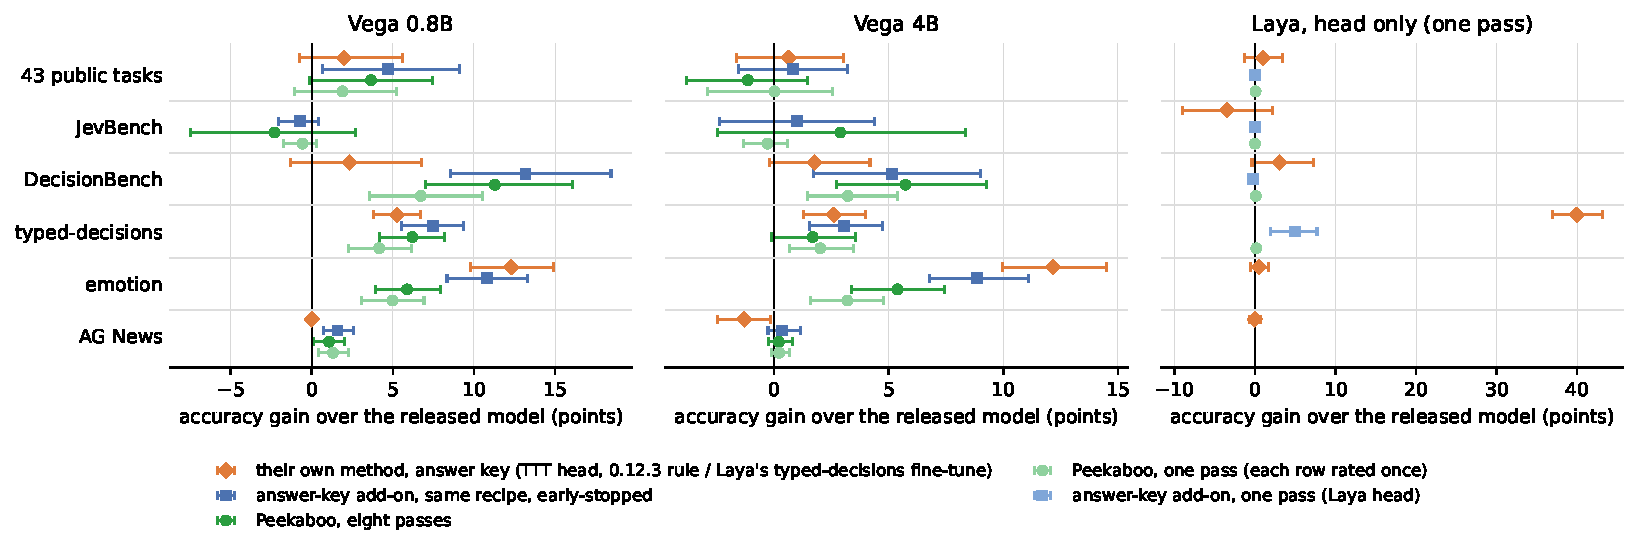
\includegraphics[width=\linewidth]{gains.pdf}
\caption{Gain over the released model on the six benchmarks, in accuracy points with 95\% intervals (seeds and row clusters resampled). Each row is a benchmark; each marker a method. Orange diamonds: the model's own labelled-data recipe (VegaML's TTT head under the 0.12.3 rule; Laya's typed-decisions fine-tune, in-domain only on typed-decisions). Blue squares: our add-on trained on the labels, early-stopped. Dark green: \pk{} with eight passes; light green: \pk{} with one pass, each row rated once. On Laya the head-only arms were run for one pass only (light blue: the labelled head, one pass). On JevBench every method is cross-fitted.}
\label{fig:gains}
\end{figure}

\begin{table}[tbp]\centering\scriptsize
\caption{Accuracy, mean over 3 seeds ($\pm$ s.d.) where a method is stochastic. JevBench has no training split: every method learns by 5-fold cross-fitting there, and pooled Peekaboo never sees it.}
\label{tab:acc}
\setlength{\tabcolsep}{2.5pt}
\resizebox{\linewidth}{!}{\begin{tabular}{llrrrrrrr}
\toprule
model & method & learns from & public & JevBench & DecisionB. & typed-dec. & emotion & AG News \\
\midrule
Vega 0.8B & released model & none & 0.556 & 0.545 & 0.509 & 0.666 & 0.568 & 0.901 \\
 & TTT head, 0.8.0 rule & answer key & 0.516 & $\cdot$ & 0.530 & 0.719 & 0.691 & 0.900 \\
 & TTT head, 0.12.3 rule & answer key & 0.576 & $\cdot$ & 0.532 & 0.719 & 0.691 & 0.901 \\
 & answer-key adapter, same recipe & answer key & 0.590 {\scriptsize$\pm$0.004} & 0.537 {\scriptsize$\pm$0.020} & 0.632 {\scriptsize$\pm$0.004} & 0.737 {\scriptsize$\pm$0.002} & 0.679 {\scriptsize$\pm$0.007} & 0.901 {\scriptsize$\pm$0.003} \\
 & answer-key adapter, early-stopped & answer key & 0.603 {\scriptsize$\pm$0.010} & 0.538 {\scriptsize$\pm$0.005} & 0.641 {\scriptsize$\pm$0.010} & 0.740 {\scriptsize$\pm$0.003} & 0.676 {\scriptsize$\pm$0.006} & 0.917 {\scriptsize$\pm$0.002} \\
 & answer-key adapter, one pass & answer key & 0.592 {\scriptsize$\pm$0.003} & 0.540 {\scriptsize$\pm$0.002} & 0.608 {\scriptsize$\pm$0.007} & 0.734 {\scriptsize$\pm$0.007} & 0.635 {\scriptsize$\pm$0.002} & 0.917 {\scriptsize$\pm$0.002} \\
 & \textbf{Peekaboo}, eight passes & verdicts & 0.593 {\scriptsize$\pm$0.013} & 0.522 {\scriptsize$\pm$0.010} & 0.622 {\scriptsize$\pm$0.002} & 0.728 {\scriptsize$\pm$0.007} & 0.627 {\scriptsize$\pm$0.004} & 0.912 {\scriptsize$\pm$0.004} \\
 & \textbf{Peekaboo}, one pass & verdicts & 0.575 {\scriptsize$\pm$0.008} & 0.540 {\scriptsize$\pm$0.002} & 0.576 {\scriptsize$\pm$0.011} & 0.708 {\scriptsize$\pm$0.003} & 0.618 {\scriptsize$\pm$0.006} & 0.914 {\scriptsize$\pm$0.002} \\
 & logged best answers, rated once & verdicts & $\cdot$ & $\cdot$ & 0.583 {\scriptsize$\pm$0.009} & 0.726 & 0.603 & $\cdot$ \\
 & Peekaboo, no KL term & verdicts & 0.582 & 0.517 {\scriptsize$\pm$0.014} & 0.609 {\scriptsize$\pm$0.004} & 0.709 & 0.622 & 0.916 \\
\addlinespace
Vega 4B & released model & none & 0.718 & 0.667 & 0.636 & 0.729 & 0.575 & 0.928 \\
 & TTT head, 0.8.0 rule & answer key & 0.678 & $\cdot$ & 0.640 & 0.757 & 0.697 & 0.915 \\
 & TTT head, 0.12.3 rule & answer key & 0.724 & $\cdot$ & 0.654 & 0.755 & 0.697 & 0.915 \\
 & answer-key adapter, same recipe & answer key & 0.706 {\scriptsize$\pm$0.002} & 0.706 {\scriptsize$\pm$0.011} & 0.687 {\scriptsize$\pm$0.007} & 0.769 {\scriptsize$\pm$0.001} & 0.640 {\scriptsize$\pm$0.001} & 0.924 {\scriptsize$\pm$0.003} \\
 & answer-key adapter, early-stopped & answer key & 0.726 {\scriptsize$\pm$0.005} & 0.677 {\scriptsize$\pm$0.010} & 0.688 {\scriptsize$\pm$0.005} & 0.760 {\scriptsize$\pm$0.008} & 0.663 {\scriptsize$\pm$0.004} & 0.931 {\scriptsize$\pm$0.004} \\
 & answer-key adapter, one pass & answer key & 0.723 {\scriptsize$\pm$0.003} & 0.667 {\scriptsize$\pm$0.000} & 0.683 {\scriptsize$\pm$0.009} & 0.775 {\scriptsize$\pm$0.008} & 0.631 {\scriptsize$\pm$0.004} & 0.931 {\scriptsize$\pm$0.003} \\
 & \textbf{Peekaboo}, eight passes & verdicts & 0.706 {\scriptsize$\pm$0.005} & 0.696 {\scriptsize$\pm$0.005} & 0.694 {\scriptsize$\pm$0.005} & 0.746 {\scriptsize$\pm$0.010} & 0.629 {\scriptsize$\pm$0.009} & 0.930 {\scriptsize$\pm$0.002} \\
 & \textbf{Peekaboo}, one pass & verdicts & 0.718 {\scriptsize$\pm$0.017} & 0.664 {\scriptsize$\pm$0.003} & 0.669 {\scriptsize$\pm$0.004} & 0.749 {\scriptsize$\pm$0.004} & 0.607 {\scriptsize$\pm$0.003} & 0.930 {\scriptsize$\pm$0.002} \\
 & logged best answers, rated once & verdicts & $\cdot$ & $\cdot$ & 0.655 {\scriptsize$\pm$0.004} & 0.769 & 0.611 & $\cdot$ \\
 & Peekaboo, no KL term & verdicts & 0.713 & 0.693 & 0.672 {\scriptsize$\pm$0.002} & 0.742 & 0.519 & 0.928 \\
\addlinespace
Laya & released model & none & 0.540 & 0.576 & 0.406 & 0.362 & 0.599 & 0.930 \\
 & laya-typed-decisions (fine-tune on typed-decisions) & answer key & 0.550 & 0.541 & 0.436 & 0.761 & 0.604 & 0.930 \\
 & answer-key head, one pass & answer key & 0.541 & 0.576 & 0.403 & 0.412 {\scriptsize$\pm$0.011} & $\cdot$ & $\cdot$ \\
 & \textbf{Peekaboo}, head only, one pass & verdicts & 0.541 & 0.576 & 0.406 & 0.364 {\scriptsize$\pm$0.003} & $\cdot$ & $\cdot$ \\
 & answer-key fine-tune, encoder unfrozen & answer key & 0.587 {\scriptsize$\pm$0.009} & 0.535 {\scriptsize$\pm$0.025} & 0.560 {\scriptsize$\pm$0.016} & 0.750 & 0.899 & $\cdot$ \\
 & answer-key fine-tune, encoder unfrozen, early-stopped & answer key & 0.584 {\scriptsize$\pm$0.003} & 0.595 {\scriptsize$\pm$0.005} & 0.554 {\scriptsize$\pm$0.005} & 0.750 & 0.905 & $\cdot$ \\
 & \textbf{Peekaboo}, encoder unfrozen, eight passes & verdicts & 0.566 {\scriptsize$\pm$0.001} & 0.558 {\scriptsize$\pm$0.030} & 0.545 {\scriptsize$\pm$0.014} & 0.685 & 0.820 & $\cdot$ \\
 & \textbf{Peekaboo}, encoder unfrozen, one pass & verdicts & 0.562 {\scriptsize$\pm$0.005} & 0.573 {\scriptsize$\pm$0.005} & 0.482 {\scriptsize$\pm$0.026} & 0.588 & 0.698 & $\cdot$ \\
\bottomrule
\end{tabular}}
\end{table}

\begin{table}[tbp]\centering\scriptsize
\caption{Gain over the released model in accuracy points, with 95\% intervals that resample seeds and row clusters; $\dagger$ marks differences that survive Holm adjustment within the method's family. JevBench has no training split: every method learns by 5-fold cross-fitting there, and pooled Peekaboo never sees it.}
\label{tab:gain}
\setlength{\tabcolsep}{2.5pt}
\resizebox{\linewidth}{!}{\begin{tabular}{llrrrrrrr}
\toprule
model & method & learns from & public & JevBench & DecisionB. & typed-dec. & emotion & AG News \\
\midrule
Vega 0.8B & released model & none & -- & -- & -- & -- & -- & -- \\
 & TTT head, 0.8.0 rule & answer key & -4.1 & $\cdot$ & +2.1 & +5.3 & +12.3 & -0.2 \\
 & TTT head, 0.12.3 rule & answer key & +2.0 & $\cdot$ & +2.3 & +5.2 & +12.3 & +0.0 \\
 & answer-key adapter, same recipe & answer key & +3.4 & -0.9 & +12.3 & +7.0 & +11.1 & +0.0 \\
 & answer-key adapter, early-stopped & answer key & +4.7 & -0.7 & +13.2 & +7.4 & +10.8 & +1.6 \\
 & answer-key adapter, one pass & answer key & +3.6 & -0.6 & +10.0 & +6.8 & +6.6 & +1.6 \\
 & \textbf{Peekaboo}, eight passes & verdicts & +3.7 & -2.3 & +11.3$^{\dagger}$ & +6.2$^{\dagger}$ & +5.9$^{\dagger}$ & +1.1 \\
 & \textbf{Peekaboo}, one pass & verdicts & +1.9 & -0.6 & +6.7$^{\dagger}$ & +4.1$^{\dagger}$ & +5.0$^{\dagger}$ & +1.3$^{\dagger}$ \\
 & logged best answers, rated once & verdicts & $\cdot$ & $\cdot$ & +7.4 & +6.0 & +3.5 & $\cdot$ \\
 & Peekaboo, no KL term & verdicts & +2.5 & -2.9 & +10.0 & +4.2 & +5.4 & +1.5 \\
\addlinespace
Vega 4B & released model & none & -- & -- & -- & -- & -- & -- \\
 & TTT head, 0.8.0 rule & answer key & -3.9 & $\cdot$ & +0.4 & +2.8 & +12.2 & -1.3 \\
 & TTT head, 0.12.3 rule & answer key & +0.6 & $\cdot$ & +1.8 & +2.6 & +12.2 & -1.3 \\
 & answer-key adapter, same recipe & answer key & -1.2 & +3.9 & +5.1 & +4.0 & +6.5 & -0.3 \\
 & answer-key adapter, early-stopped & answer key & +0.8 & +1.0 & +5.1 & +3.0 & +8.8 & +0.3 \\
 & answer-key adapter, one pass & answer key & +0.5 & -0.0 & +4.7 & +4.6 & +5.7 & +0.3 \\
 & \textbf{Peekaboo}, eight passes & verdicts & -1.1 & +2.9 & +5.7$^{\dagger}$ & +1.7 & +5.4$^{\dagger}$ & +0.2 \\
 & \textbf{Peekaboo}, one pass & verdicts & +0.0 & -0.3 & +3.2$^{\dagger}$ & +2.0$^{\dagger}$ & +3.2$^{\dagger}$ & +0.2 \\
 & logged best answers, rated once & verdicts & $\cdot$ & $\cdot$ & +1.8 & +4.0 & +3.6 & $\cdot$ \\
 & Peekaboo, no KL term & verdicts & -0.5 & +2.6 & +3.5 & +1.3 & -5.6 & +0.0 \\
\addlinespace
Laya & released model & none & -- & -- & -- & -- & -- & -- \\
 & laya-typed-decisions (fine-tune on typed-decisions) & answer key & +1.0 & -3.5 & +3.1 & +40.0 & +0.5 & +0.0 \\
 & answer-key head, one pass & answer key & +0.1 & +0.0 & -0.3 & +5.0 & $\cdot$ & $\cdot$ \\
 & \textbf{Peekaboo}, head only, one pass & verdicts & +0.1 & +0.0 & +0.1 & +0.2 & $\cdot$ & $\cdot$ \\
 & answer-key fine-tune, encoder unfrozen & answer key & +4.6 & -4.0 & +15.4 & +38.8 & +30.0 & $\cdot$ \\
 & answer-key fine-tune, encoder unfrozen, early-stopped & answer key & +4.3 & +1.9 & +14.8 & +38.8 & +30.6 & $\cdot$ \\
 & \textbf{Peekaboo}, encoder unfrozen, eight passes & verdicts & +2.6 & -1.7 & +14.0$^{\dagger}$ & +32.3$^{\dagger}$ & +22.2$^{\dagger}$ & $\cdot$ \\
 & \textbf{Peekaboo}, encoder unfrozen, one pass & verdicts & +2.1 & -0.3 & +7.7 & +22.6 & +9.9 & $\cdot$ \\
\bottomrule
\end{tabular}}
\end{table}

\begin{table}[tbp]\centering\scriptsize
\caption{Head to head, in accuracy points with 95\% intervals (seeds and row clusters resampled). Positive means the first method is better. $\dagger$: survives Holm adjustment within the row's family; NI: non-inferior at a 2-point margin (lower bound above $-2$). TTT is scored under the vegaml 0.12.3 rule; for Laya ``their method'' is the typed-decisions fine-tune, in-domain only on typed-decisions.}
\label{tab:h2h}
\setlength{\tabcolsep}{3pt}
\resizebox{\linewidth}{!}{\begin{tabular}{llrrrrrr}
\toprule
model & comparison & public & JevBench & DecisionB. & typed-dec. & emotion & AG News \\
\midrule
\multicolumn{8}{l}{\textit{Vega 0.8B}} \\
 & Peekaboo (8 passes) vs. their method & +1.7 {\scriptsize[-1.6, +5.0]} & -- & +9.0 {\scriptsize[+5.4, +12.6]} & +0.9 {\scriptsize[-0.7, +2.7]} & -6.4 {\scriptsize[-8.4, -4.3]} & +1.1 {\scriptsize[+0.1, +2.0]} \\
 & Peekaboo (8) vs. answer key, same recipe (8) & +0.3 {\scriptsize[-2.8, +3.6]} & -1.4 {\scriptsize[-6.1, +3.0]} & -1.0 {\scriptsize[-3.0, +1.0]} & -0.9 {\scriptsize[-2.2, +0.5]} & -5.2 {\scriptsize[-7.1, -3.3]}$^{\dagger}$ & +1.0 {\scriptsize[-0.1, +2.1]} NI \\
 & Peekaboo (8) vs. answer key, early-stopped & -1.1 {\scriptsize[-4.0, +2.0]} & -1.6 {\scriptsize[-7.0, +3.5]} & -1.9 {\scriptsize[-4.1, +0.3]} & -1.3 {\scriptsize[-2.6, +0.1]} & -4.9 {\scriptsize[-6.8, -3.0]} & -0.5 {\scriptsize[-1.3, +0.2]} NI \\
 & Peekaboo (1 pass) vs. answer key (1 pass) & -1.7 {\scriptsize[-3.7, +0.5]} & -0.0 {\scriptsize[-1.0, +1.0]} NI & -3.2 {\scriptsize[-5.8, -0.6]} & -2.7 {\scriptsize[-4.1, -1.2]} & -1.7 {\scriptsize[-3.0, -0.4]} & -0.3 {\scriptsize[-0.9, +0.4]} NI \\
 & Peekaboo, 1 pass vs. 8 passes & -1.8 {\scriptsize[-4.4, +0.8]} & +1.7 {\scriptsize[-3.2, +7.2]} & -4.6 {\scriptsize[-8.1, -1.4]} & -2.1 {\scriptsize[-3.6, -0.4]} & -0.9 {\scriptsize[-2.4, +0.5]} & +0.2 {\scriptsize[-0.5, +1.0]} \\
 & logged best answers vs. Peekaboo (1 pass) & -- & -- & +0.7 {\scriptsize[-2.4, +3.7]} & +1.9 {\scriptsize[+0.3, +3.5]} NI & -1.5 {\scriptsize[-4.1, +0.7]} & -- \\
 & KL term vs. none & +1.1 {\scriptsize[-1.5, +3.9]} & +0.6 {\scriptsize[-2.4, +3.7]} & +1.2 {\scriptsize[-0.6, +3.0]} & +1.9 {\scriptsize[+0.3, +3.5]} & +0.5 {\scriptsize[-1.0, +1.8]} & -0.5 {\scriptsize[-1.3, +0.3]} \\
 & with the switch vs. without & +0.0 {\scriptsize[-2.2, +2.3]} & +2.3 {\scriptsize[-2.9, +7.7]} & +0.0 {\scriptsize[-1.2, +1.1]} & +0.0 {\scriptsize[-1.2, +1.3]} & +0.0 {\scriptsize[-1.1, +1.1]} & +0.0 {\scriptsize[-0.7, +0.7]} \\
\midrule
\multicolumn{8}{l}{\textit{Vega 4B}} \\
 & Peekaboo (8 passes) vs. their method & -1.8 {\scriptsize[-4.3, +0.7]} & -- & +4.0 {\scriptsize[+1.5, +6.5]} & -0.9 {\scriptsize[-2.6, +0.9]} & -6.8 {\scriptsize[-8.9, -4.7]} & +1.5 {\scriptsize[+0.4, +2.6]} \\
 & Peekaboo (8) vs. answer key, same recipe (8) & +0.0 {\scriptsize[-2.0, +2.0]} & -1.0 {\scriptsize[-5.0, +2.8]} & +0.6 {\scriptsize[-1.6, +2.7]} NI & -2.3 {\scriptsize[-3.8, -0.8]}$^{\dagger}$ & -1.1 {\scriptsize[-3.2, +1.0]} & +0.6 {\scriptsize[-0.1, +1.3]} NI \\
 & Peekaboo (8) vs. answer key, early-stopped & -2.0 {\scriptsize[-4.0, -0.2]} & +1.9 {\scriptsize[-2.7, +6.6]} & +0.6 {\scriptsize[-1.2, +2.3]} NI & -1.4 {\scriptsize[-2.9, +0.4]} & -3.5 {\scriptsize[-5.3, -1.7]} & -0.1 {\scriptsize[-0.8, +0.5]} NI \\
 & Peekaboo (1 pass) vs. answer key (1 pass) & -0.5 {\scriptsize[-3.0, +1.4]} & -0.3 {\scriptsize[-1.4, +0.7]} NI & -1.4 {\scriptsize[-3.8, +0.8]} & -2.6 {\scriptsize[-4.0, -1.2]} & -2.5 {\scriptsize[-3.7, -1.2]} & -0.1 {\scriptsize[-0.7, +0.5]} NI \\
 & Peekaboo, 1 pass vs. 8 passes & +1.2 {\scriptsize[-1.3, +3.5]} & -3.2 {\scriptsize[-8.7, +2.4]} & -2.5 {\scriptsize[-5.8, +0.0]} & +0.3 {\scriptsize[-1.2, +1.9]} & -2.2 {\scriptsize[-3.8, -0.5]} & +0.0 {\scriptsize[-0.6, +0.5]} \\
 & logged best answers vs. Peekaboo (1 pass) & -- & -- & -1.4 {\scriptsize[-4.4, +1.9]} & +2.0 {\scriptsize[+0.7, +3.4]} NI & +0.4 {\scriptsize[-1.9, +2.6]} NI & -- \\
 & KL term vs. none & -0.6 {\scriptsize[-2.8, +1.4]} & +0.3 {\scriptsize[-3.1, +3.8]} & +2.2 {\scriptsize[+0.4, +4.2]} & +0.4 {\scriptsize[-1.5, +2.3]} & +11.0 {\scriptsize[+8.5, +13.5]}$^{\dagger}$ & +0.2 {\scriptsize[-0.2, +0.8]} \\
 & with the switch vs. without & +0.0 {\scriptsize[-1.3, +1.2]} & -2.7 {\scriptsize[-8.1, +2.5]} & +0.0 {\scriptsize[-1.1, +1.2]} & -0.7 {\scriptsize[-3.0, +1.5]} & +0.0 {\scriptsize[-1.5, +1.6]} & +0.0 {\scriptsize[-0.5, +0.4]} \\
\midrule
\multicolumn{8}{l}{\textit{Laya}} \\
 & Peekaboo, head (1) vs. answer-key head (1) & +0.0 {\scriptsize[-0.3, +0.3]} NI & +0.0 {\scriptsize[+0.0, +0.0]} NI & +0.4 {\scriptsize[+0.1, +0.7]} NI & -4.8 {\scriptsize[-7.5, -2.0]} & -- & -- \\
 & Peekaboo, encoder (8) vs. their fine-tune & +1.6 {\scriptsize[-2.1, +5.3]} & +1.7 {\scriptsize[-4.7, +8.8]} & +10.9 {\scriptsize[+4.7, +16.7]}$^{\dagger}$ & -7.6 {\scriptsize[-9.8, -5.4]}$^{\dagger}$ & +21.6 {\scriptsize[+19.4, +24.0]}$^{\dagger}$ & -- \\
 & Peekaboo, encoder (8) vs. answer-key encoder, same recipe & -2.1 {\scriptsize[-5.1, +0.7]} & +2.3 {\scriptsize[-3.9, +7.9]} & -1.4 {\scriptsize[-5.1, +2.0]} & -6.5 {\scriptsize[-8.7, -4.1]}$^{\dagger}$ & -7.9 {\scriptsize[-9.6, -6.1]}$^{\dagger}$ & -- \\
 & Peekaboo, encoder (8) vs. answer-key encoder, early-stopped & -1.8 {\scriptsize[-4.7, +0.9]} & -3.6 {\scriptsize[-8.7, +1.4]} & -0.9 {\scriptsize[-4.5, +2.0]} & -6.5 {\scriptsize[-8.7, -4.3]} & -8.4 {\scriptsize[-10.2, -6.7]} & -- \\
 & Peekaboo, encoder: 1 pass vs. 8 & -0.4 {\scriptsize[-3.0, +2.1]} & +1.4 {\scriptsize[-4.4, +6.9]} & -6.3 {\scriptsize[-11.1, -1.9]} & -9.7 {\scriptsize[-12.1, -7.1]} & -12.2 {\scriptsize[-14.2, -10.3]} & -- \\
\bottomrule
\end{tabular}}
\end{table}


Tables~\ref{tab:acc} and \ref{tab:gain} give accuracy and gain over the released model for every arm, Table~\ref{tab:h2h} the paired head-to-heads, and Figure~\ref{fig:gains} the picture. Under the eight-pass protocol the verdict-trained add-on lands close to the same add-on trained on labels and early-stopped, and mostly below it. On DecisionBench \pk{} gains $\gainSmallPkDb$ points at 0.8B and $\gainBigPkDb$ at 4B; the early-stopped labelled adapter gains $\gainSmallSupEsDb$ and $\gainBigSupEsDb$. The paired difference is $\gainSmallPkDbVsSupEs$ $\ciSmallPkDbVsSupEs$ at 0.8B and $\gainBigPkDbVsSupEs$ $\ciBigPkDbVsSupEs$ at 4B; on typed-decisions $\gainSmallPkTypedVsSupEs$ and $\gainBigPkTypedVsSupEs$, on the public menu $\gainSmallPkPubVsSupEs$ and $\gainBigPkPubVsSupEs$, on AG News $\gainSmallPkAgVsSupEs$ and $\gainBigPkAgVsSupEs$, on JevBench $\gainSmallPkJevVsSupEs$ and $\gainBigPkJevVsSupEs$. Emotion is the exception: $\gainSmallPkEmoVsSupEs$ $\ciSmallPkEmoVsSupEs$ and $\gainBigPkEmoVsSupEs$ $\ciBigPkEmoVsSupEs$, and these two are the only differences in the family that survive Holm adjustment. Against the same-recipe adapter without early stopping the differences are smaller still. This is what the $\pi(y)$ weighting predicts for a protocol that reveals most labels (Section~\ref{sec:anatomy}): the two arms then optimise nearly the same objective. The first version read these gaps as ``the bit is nearly as good as the label''; the accurate reading is that eight rounds of verdicts on the same rows are nearly as good as the labels, because they mostly are the labels. The one-rating arms below measure a single verdict.

\paragraph{Against VegaML's TTT head.}
Under the 0.12.3 rule, which keeps a head only where it beats the engine on its own fit rows, the TTT head gains $\gainSmallTttGuardPub$ and $\gainBigTttGuardPub$ on the public menu; under the 0.8.0 rule it lost $\absSmallTttPub$ and $\absBigTttPub$ points, the losses our first version counted as wins. \pk{} minus the guarded TTT head is $\gainSmallPkDbVsTttGuard$ $\ciSmallPkDbVsTttGuard$ on DecisionBench at 0.8B and $\gainBigPkDbVsTttGuard$ $\ciBigPkDbVsTttGuard$ at 4B; $\gainSmallPkAgVsTttGuard$ $\ciSmallPkAgVsTttGuard$ and $\gainBigPkAgVsTttGuard$ $\ciBigPkAgVsTttGuard$ on AG News; $\gainSmallPkPubVsTttGuard$ $\ciSmallPkPubVsTttGuard$ and $\gainBigPkPubVsTttGuard$ $\ciBigPkPubVsTttGuard$ on the public menu; $\gainSmallPkTypedVsTttGuard$ and $\gainBigPkTypedVsTttGuard$ on typed-decisions; and $\gainSmallPkEmoVsTttGuard$ $\ciSmallPkEmoVsTttGuard$ and $\gainBigPkEmoVsTttGuard$ $\ciBigPkEmoVsTttGuard$ on emotion. After Holm adjustment the verdict-trained adapter is ahead of VegaML's labelled recipe on DecisionBench at both sizes and on AG News at 4B, level on the public menu and typed-decisions, and behind on emotion at both sizes. On DecisionBench the guarded head answers $\tttCoveredSmallDb$ of 1,075 rows at 0.8B and $\tttCoveredBigDb$ at 4B (Table~\ref{tab:ttt}). On the rows it answers, \pk{} minus TTT is $\gainPeekabooVsTttCoveredSmallDb$ $\ciPeekabooVsTttCoveredSmallDb$ and $\gainPeekabooVsTttCoveredBigDb$ $\ciPeekabooVsTttCoveredBigDb$, neither significant, and the labelled adapter does about as well there ($\gainAdapterVsTttCoveredSmallDb$, $\gainAdapterVsTttCoveredBigDb$). The significant margin is on the rows the head leaves to the engine ($\gainPeekabooVsTttUncoveredSmallDb$ and $\gainPeekabooVsTttUncoveredBigDb$), where it is a comparison with the released model, and it belongs to an in-engine adapter that reads the option text, not to the feedback signal. Emotion goes to TTT by a wide margin: a six-way single-label task with 3,200 labelled rows is where a logistic head on good features is at its best.

\paragraph{JevBench.}
With every arm cross-fitted, the answer-key adapter is defined on JevBench too, which removes the first version's claim that \pk{} was the only method to improve Vega 4B there. At 4B \pk{} gains $\gainBigPkJev$ $\ciBigPkJev$ and the labelled adapter $\gainBigSupJev$ $\ciBigSupJev$; at 0.8B \pk{} loses $\absSmallPkJev$ points and the labelled adapter $\absSmallSupJev$. None of these intervals excludes zero. JevBench has 231 rows and 38-to-42-row calibration folds.

\subsection{One rating per row, and feedback as a deployment delivers it}
\label{sec:realistic}

\begin{figure}[t]\centering
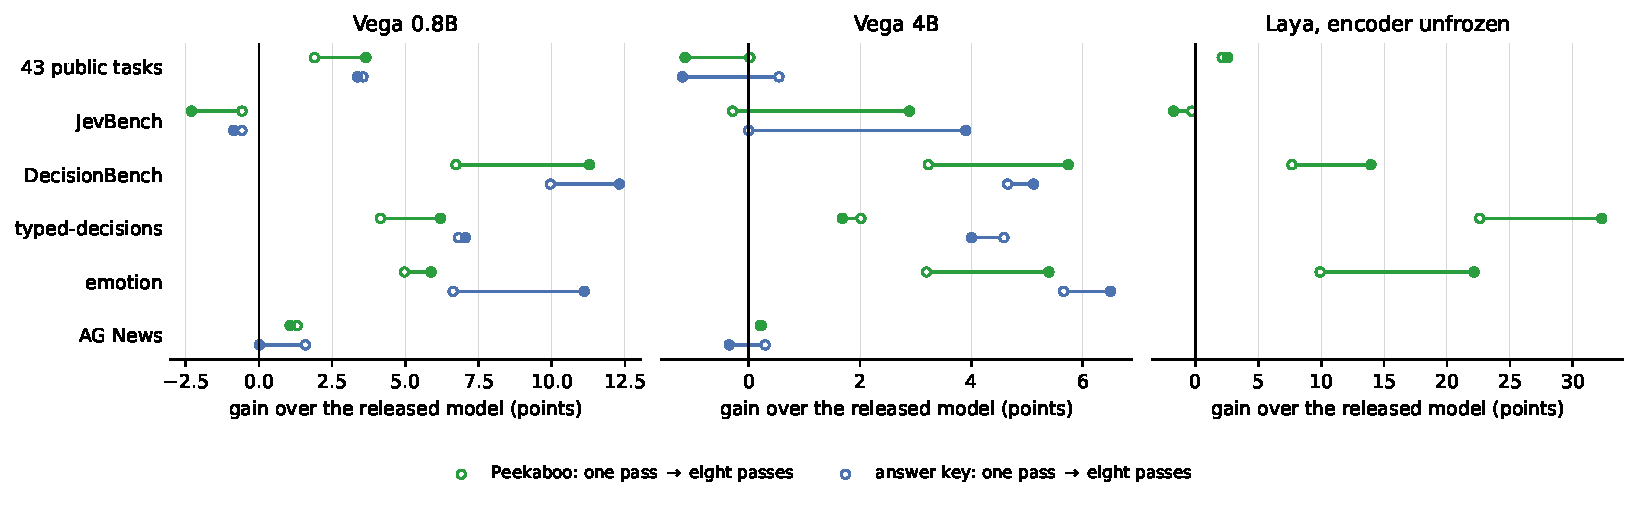
\includegraphics[width=\linewidth]{passes.pdf}
\caption{One pass (open markers) against eight (filled), for \pk{} (green) and the answer-key add-on (blue), as gain over the released model. One pass rates each row once and takes one eighth of the gradient steps. Laya: the encoder-unfrozen \pk{} only.}
\label{fig:passes}
\end{figure}

\begin{table}[tbp]\centering\small
\caption{Feedback as a deployment delivers it: gain over the released model in points (95\% intervals), on the three benchmarks with the realistic-feedback arms.}
\label{tab:realistic}
\setlength{\tabcolsep}{3pt}
\resizebox{\linewidth}{!}{\begin{tabular}{lrrrrrrrrr}
\toprule
feedback & \multicolumn{3}{c}{DecisionBench} & \multicolumn{3}{c}{typed-decisions} & \multicolumn{3}{c}{emotion} \\
 & Vega 0.8B & Vega 4B & Laya (head) & Vega 0.8B & Vega 4B & Laya (head) & Vega 0.8B & Vega 4B & Laya (head) \\
\midrule
eight passes, clean verdicts & +11.3 {\scriptsize[+7.0, +16.1]} & +5.7 {\scriptsize[+2.7, +9.3]} & -- & +6.2 {\scriptsize[+4.2, +8.2]} & +1.7 {\scriptsize[-0.1, +3.6]} & -- & +5.9 {\scriptsize[+3.9, +8.0]} & +5.4 {\scriptsize[+3.4, +7.4]} & -- \\
one pass, clean verdicts & +6.7 {\scriptsize[+3.6, +10.5]} & +3.2 {\scriptsize[+1.5, +5.4]} & +0.1 {\scriptsize[+0.0, +0.3]} & +4.1 {\scriptsize[+2.2, +6.1]} & +2.0 {\scriptsize[+0.7, +3.5]} & +0.2 {\scriptsize[-0.2, +0.5]} & +5.0 {\scriptsize[+3.1, +6.9]} & +3.2 {\scriptsize[+1.6, +4.8]} & -- \\
logged: the released model's best answers, rated once & +7.4 {\scriptsize[+3.4, +12.2]} & +1.8 {\scriptsize[-1.4, +5.3]} & -- & +6.0 {\scriptsize[+3.9, +8.2]} & +4.0 {\scriptsize[+2.5, +5.7]} & -- & +3.5 {\scriptsize[+0.7, +6.2]} & +3.6 {\scriptsize[+1.2, +5.9]} & -- \\
logged: the released model's sampled answers, rated once (clipped IPS) & +8.3 {\scriptsize[+4.4, +13.0]} & +4.3 {\scriptsize[+1.6, +7.3]} & -- & +5.6 {\scriptsize[+3.5, +7.6]} & +1.8 {\scriptsize[+0.1, +3.8]} & -- & +6.6 {\scriptsize[+4.6, +8.6]} & +4.5 {\scriptsize[+2.5, +6.6]} & -- \\
20\% of verdicts flipped (eight passes) & +9.1 {\scriptsize[+5.8, +12.8]} & +4.2 {\scriptsize[+1.7, +7.3]} & -- & +5.9 {\scriptsize[+4.2, +7.5]} & +2.8 {\scriptsize[+1.2, +4.3]} & -- & +4.7 {\scriptsize[+3.1, +6.3]} & +4.7 {\scriptsize[+2.7, +6.8]} & -- \\
half of the answers rated (eight passes) & +10.3 {\scriptsize[+6.2, +14.8]} & +4.7 {\scriptsize[+1.6, +8.3]} & -- & +5.2 {\scriptsize[+3.1, +7.5]} & +3.5 {\scriptsize[+1.8, +5.3]} & -- & +6.5 {\scriptsize[+4.2, +8.9]} & +0.0 {\scriptsize[+0.0, +0.0]} & -- \\
every wrong answer reported, 20\% of right ones (eight passes) & +10.0 {\scriptsize[+6.0, +14.7]} & +5.7 {\scriptsize[+2.7, +9.1]} & -- & +7.0 {\scriptsize[+5.0, +9.0]} & +4.2 {\scriptsize[+2.4, +5.9]} & -- & +6.7 {\scriptsize[+4.5, +9.0]} & +2.7 {\scriptsize[+0.9, +4.5]} & -- \\
answer key, one pass & +10.0 {\scriptsize[+6.3, +13.9]} & +4.7 {\scriptsize[+2.1, +7.4]} & -0.3 {\scriptsize[-0.7, +0.0]} & +6.8 {\scriptsize[+4.8, +8.8]} & +4.6 {\scriptsize[+3.0, +6.4]} & +5.0 {\scriptsize[+1.9, +7.7]} & +6.6 {\scriptsize[+4.5, +8.8]} & +5.7 {\scriptsize[+3.8, +7.7]} & -- \\
answer key, eight passes & +12.3 {\scriptsize[+7.8, +17.5]} & +5.1 {\scriptsize[+1.4, +9.1]} & -- & +7.0 {\scriptsize[+5.0, +9.1]} & +4.0 {\scriptsize[+2.5, +5.6]} & -- & +11.1 {\scriptsize[+8.6, +13.6]} & +6.5 {\scriptsize[+4.3, +8.8]} & -- \\
\bottomrule
\end{tabular}}
\end{table}


\begin{figure}[t]\centering
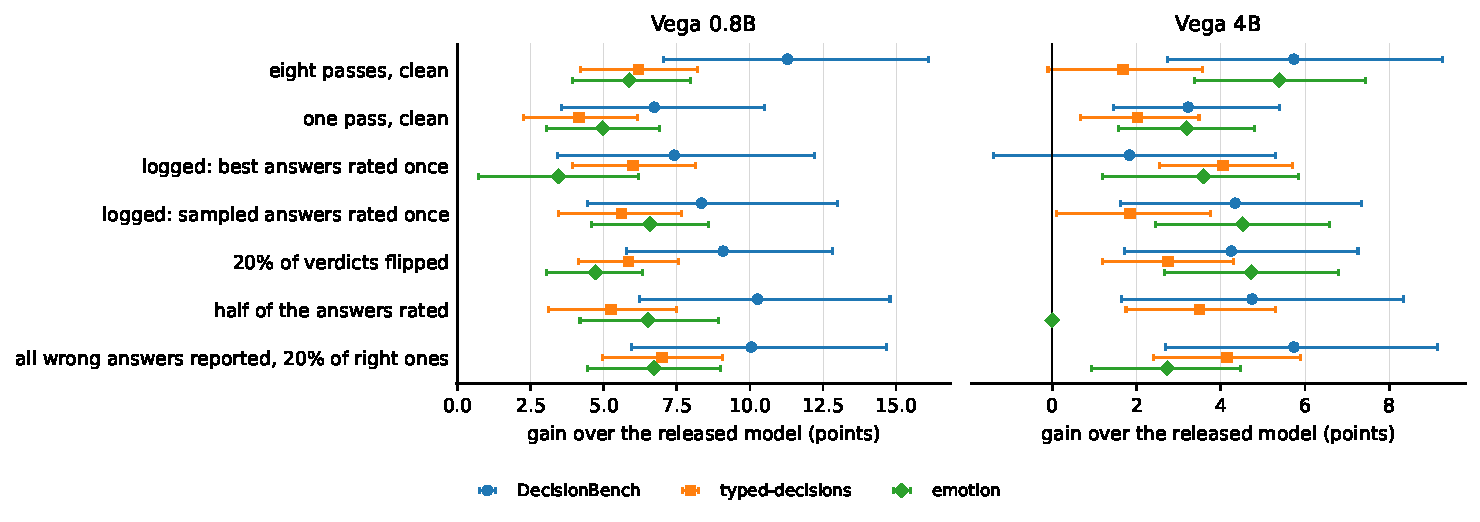
\includegraphics[width=\linewidth]{realistic.pdf}
\caption{Feedback as a deployment delivers it, on Vega: gain over the released model with 95\% intervals for the clean eight-pass and one-pass arms, the two logged arms (one verdict per row on the released model's best or sampled answers, trained off-policy), and eight-pass \pk{} with flipped, missing or complaint-skewed verdicts. The clean arms have three seeds everywhere; the logged and damaged-feedback arms three on DecisionBench and one on typed-decisions and emotion. The half-rated emotion run at 4B failed (Section~\ref{sec:realistic}).}
\label{fig:realistic}
\end{figure}

Figure~\ref{fig:passes} shows what a single pass keeps. On DecisionBench one-pass \pk{} gains $\gainSmallPkOneDb$ $\ciSmallPkOneDb$ at 0.8B and $\gainBigPkOneDb$ $\ciBigPkOneDb$ at 4B, against $\gainSmallPkDb$ and $\gainBigPkDb$ with eight passes; the one-pass labelled adapter gains $\gainSmallSupOneDb$ and $\gainBigSupOneDb$. At matched epochs the gap between verdicts and labels is $\gainSmallPkOneDbVsSupOne$ $\ciSmallPkOneDbVsSupOne$ and $\gainBigPkOneDbVsSupOne$ $\ciBigPkOneDbVsSupOne$, wider than with eight passes. On typed-decisions one pass gives $\gainSmallPkOneTyped$ and $\gainBigPkOneTyped$ (labels: $\gainSmallSupOneTyped$, $\gainBigSupOneTyped$; verdicts significantly behind at both sizes); on the public menu $\gainSmallPkOnePub$ and $\gainBigPkOnePub$; on emotion $\gainSmallPkOneEmo$ and $\gainBigPkOneEmo$; on AG News $\gainSmallPkOneAg$ and $\gainBigPkOneAg$. One pass keeps about half to two thirds of the eight-pass gain on DecisionBench and the public menu and more on emotion.

One pass confounds two things: each row is rated once, and the model takes one eighth of the gradient steps. The logged arms separate them. Each row of the pool is answered once by the released model, rated once, and the add-on is then trained on that fixed log for eight passes, off-policy. With the released model's sampled answers and clipped importance weights this gains $\gainSmallLogIpsDb$ $\ciSmallLogIpsDb$ on DecisionBench at 0.8B and $\gainBigLogIpsDb$ $\ciBigLogIpsDb$ at 4B. Against one on-policy pass that is $\gainSmallLogIpsDbVsPkOne$ $\ciSmallLogIpsDbVsPkOne$ and $\gainBigLogIpsDbVsPkOne$ $\ciBigLogIpsDbVsPkOne$; against eight passes it is $\gainSmallLogIpsDbVsPk$ $\ciSmallLogIpsDbVsPk$ and $\gainBigLogIpsDbVsPk$ $\ciBigLogIpsDbVsPk$. So on DecisionBench, where the logged arms have three seeds, more optimisation recovers part of the one-pass shortfall and the larger part, the only significant one at 0.8B, is information: more verdicts per row. On typed-decisions and emotion, where the logged arms have one seed, the logged arm is level with eight on-policy passes ($\gainSmallLogIpsTypedVsPk$ and $\gainSmallLogIpsEmoVsPk$ at 0.8B, $\gainBigLogIpsTypedVsPk$ and $\gainBigLogIpsEmoVsPk$ at 4B). Against the early-stopped labelled adapter the logged sampled arm is $\gainSmallLogIpsDbVsSupEs$ $\ciSmallLogIpsDbVsSupEs$ on DecisionBench, $\gainSmallLogIpsTypedVsSupEs$ on typed-decisions and $\gainSmallLogIpsEmoVsSupEs$ on emotion at 0.8B, and $\gainBigLogIpsDbVsSupEs$, $\gainBigLogIpsTypedVsSupEs$ and $\gainBigLogIpsEmoVsSupEs$ at 4B: one logged verdict per row stays below the labels on every cell, significantly on four of the six.

Table~\ref{tab:realistic} and Figure~\ref{fig:realistic} collect the deployment question. A system that serves its best answer rather than a sample logs only that answer's verdict: a 1 is a label, a 0 rules one option out. Learning from that log gains $\gainSmallLogArgDb$ $\ciSmallLogArgDb$ on DecisionBench at 0.8B and $\gainBigLogArgDb$ $\ciBigLogArgDb$ at 4B, $\gainSmallLogArgTyped$ and $\gainBigLogArgTyped$ on typed-decisions, and $\gainSmallLogArgEmo$ and $\gainBigLogArgEmo$ on emotion. It trails the early-stopped labels by $\absSmallLogArgDbVsSupEs$ and $\absBigLogArgDbVsSupEs$ points on DecisionBench and by $\absSmallLogArgEmoVsSupEs$ and $\absBigLogArgEmoVsSupEs$ on emotion, and on typed-decisions at 4B it is level with them ($\gainBigLogArgTypedVsSupEs$). Neither logging policy dominates: sampled answers are worth $\gainSmallLogIpsDbVsLogArg$ and $\gainBigLogIpsDbVsLogArg$ points more on DecisionBench and $\gainSmallLogIpsEmoVsLogArg$ on emotion at 0.8B, and $\gainBigLogIpsTypedVsLogArg$ on typed-decisions at 4B.

We measured damaged feedback only under the eight-pass protocol, where a flipped or missing verdict on one pass is redrawn on the next; how noise affects a single rating per row is not measured here. On DecisionBench, with three seeds, 20\% of verdicts flipped costs $\absSmallNoiseDbVsPk$ points at 0.8B and $\absBigNoiseDbVsPk$ at 4B, half of the answers unrated $\absSmallHalfDbVsPk$ and $\absBigHalfDbVsPk$, and complaint-skewed verdicts $\absSmallComplDbVsPk$ and $\absBigComplDbVsPk$. On typed-decisions and emotion these arms have one seed against the clean arm's three and differ from it by up to three points in either direction. One run failed: with half of the answers unrated on emotion at 4B the adapter's predictions are identical to the released model's on every test row and its reward stays flat through all eight passes, so that cell ($\gainBigHalfEmo$) says nothing about missing feedback. Rewards are computed from the gold answer in all of these; a rater who is systematically wrong about what was right is not simulated beyond the flipped verdicts.

\subsection{What the gain is made of}
\label{sec:anatomy}

\begin{figure}[t]\centering
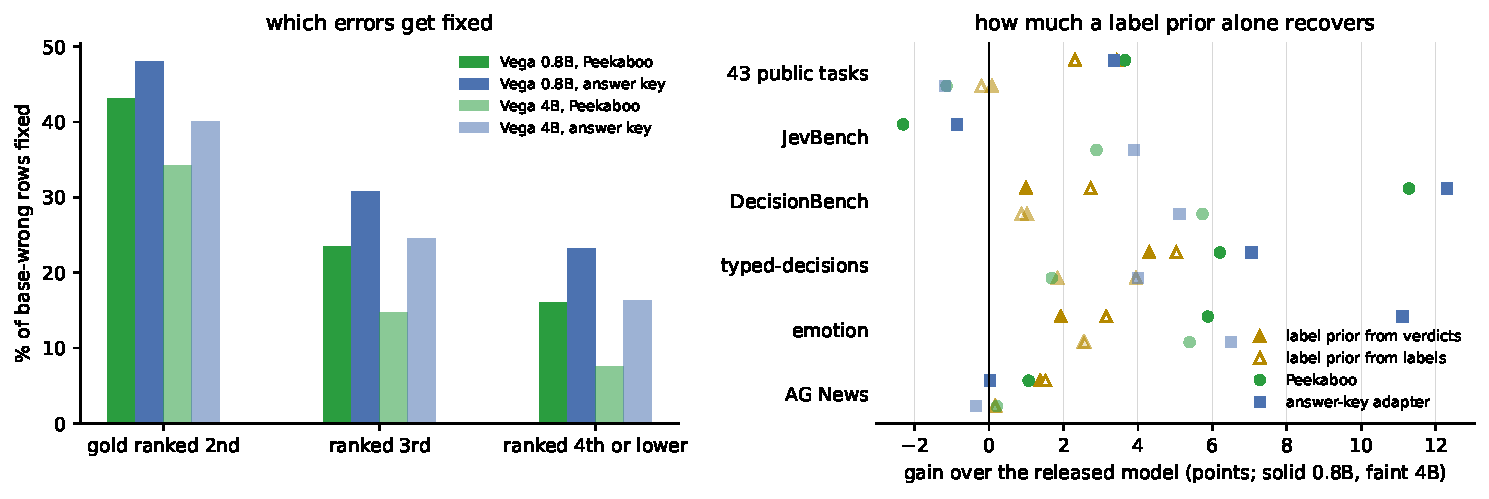
\includegraphics[width=\linewidth]{anatomy.pdf}
\caption{Left: share of the released model's wrong rows that eight-pass \pk{} and the answer-key adapter fix, by the released model's rank of the gold option (mean over benchmarks). Right: gain over the released model of a per-task label prior with no input features, trained from verdicts (filled triangles) or labels (open), beside \pk{} and the answer-key adapter.}
\label{fig:anatomy}
\end{figure}

\begin{table}[tbp]\centering\scriptsize
\caption{What the gain is made of. Left: gain over the released model of a per-task label prior with no input features (log-offsets on the released probabilities), trained from verdicts with Peekaboo's loop and from labels; and Peekaboo minus that prior. Right: how often eight on-policy passes reveal the gold answer: reward-1 events per training row (each one names the gold answer), the share of rows the base policy would reveal in 8 draws, the share of two-option rows, and the first pass's reward against the released model's best-answer accuracy on the same rows.}
\label{tab:anatomy}
\setlength{\tabcolsep}{2.5pt}
\resizebox{\linewidth}{!}{\begin{tabular}{llrrrr|rrrrr}
\toprule
model & benchmark & prior (verdicts) & prior (labels) & Peekaboo $-$ prior & params & reveals / row & $P$(revealed, 8 draws) & 2-option rows & pass-1 reward & base best-answer acc. \\
\midrule
Vega 0.8B & 43 public tasks & +3.4 & +2.3 & +0.2 {\scriptsize[-3.0, +3.1]} & 536 & 5.1 & 0.88 & 30\% & 0.50 & 0.55 \\
 & JevBench & -- & -- & -- & -- & 4.7 & -- & -- & 0.49 & -- \\
 & DecisionBench & +1.0 & +2.7 & +10.3 {\scriptsize[+6.3, +14.7]} & 28584 & 4.9 & 0.76 & 21\% & 0.48 & 0.50 \\
 & typed-decisions & +4.3 & +5.0 & +1.9 {\scriptsize[+0.1, +3.6]} & 71 & 6.1 & 0.94 & 30\% & 0.72 & 0.72 \\
 & emotion & +1.9 & +3.1 & +3.9 {\scriptsize[+2.1, +5.7]} & 6 & 4.9 & 0.85 & 0\% & 0.57 & 0.56 \\
 & AG News & +1.4 & +1.5 & -0.3 {\scriptsize[-1.2, +0.5]} & 4 & 7.5 & 0.97 & 0\% & 0.92 & 0.92 \\
\midrule
Vega 4B & 43 public tasks & +0.1 & -0.2 & -1.2 {\scriptsize[-3.6, +0.9]} & 536 & 6.1 & 0.92 & 30\% & 0.68 & 0.70 \\
 & JevBench & -- & -- & -- & -- & 5.9 & -- & -- & 0.64 & -- \\
 & DecisionBench & +1.0 & +0.9 & +4.7 {\scriptsize[+2.0, +7.8]} & 28584 & 5.6 & 0.82 & 21\% & 0.62 & 0.61 \\
 & typed-decisions & +1.8 & +3.9 & -0.2 {\scriptsize[-1.8, +1.6]} & 71 & 6.4 & 0.96 & 30\% & 0.75 & 0.79 \\
 & emotion & +2.5 & +2.6 & +2.9 {\scriptsize[+1.1, +4.7]} & 6 & 4.8 & 0.84 & 0\% & 0.57 & 0.57 \\
 & AG News & +0.2 & +0.2 & +0.0 {\scriptsize[-0.4, +0.6]} & 4 & 7.4 & 0.96 & 0\% & 0.92 & 0.93 \\
\midrule
Laya & typed-decisions & +15.3 & +17.4 & -- & 71 & -- & -- & -- & -- & -- \\
 & emotion & -1.4 & -3.3 & -- & 6 & -- & -- & -- & -- & -- \\
 & AG News & -0.6 & -0.1 & -- & 4 & -- & -- & -- & -- & -- \\
\bottomrule
\end{tabular}}
\end{table}

\begin{table}[tbp]\centering\small
\caption{Which rows change. Share of the released model's wrong rows that a method fixes, by the released model's rank of the gold option, and share of its right rows the method breaks (mean over benchmarks with a training split and over seeds).}
\label{tab:fixbreak}
\begin{tabular}{llrrrrr}
\toprule
model & method & fixed, all & gold 2nd & gold 3rd & gold 4th+ & broken \\
\midrule
Vega 0.8B & Peekaboo (8 passes) & 32\% & 43\% & 23\% & 13\% & 11\% \\
Vega 0.8B & Peekaboo (1 pass) & 26\% & 37\% & 13\% & 9\% & 8\% \\
Vega 0.8B & answer key (8 passes) & 40\% & 48\% & 31\% & 23\% & 13\% \\
Vega 4B & Peekaboo (8 passes) & 25\% & 34\% & 15\% & 8\% & 8\% \\
Vega 4B & Peekaboo (1 pass) & 18\% & 27\% & 9\% & 4\% & 6\% \\
Vega 4B & answer key (8 passes) & 32\% & 40\% & 25\% & 16\% & 10\% \\
Laya & Peekaboo (1 pass) & 0\% & 1\% & 0\% & 0\% & 0\% \\
Laya & Peekaboo, encoder (8) & 47\% & 58\% & 45\% & 32\% & 16\% \\
Laya & answer-key encoder (8) & 55\% & 65\% & 55\% & 44\% & 15\% \\
\bottomrule
\end{tabular}
\end{table}

\begin{table}[tbp]\centering\small
\caption{VegaML's TTT head answers a row only where a head was kept for its task and the option set matches (``covered''); elsewhere its output is the released engine's. Eight-pass Peekaboo minus TTT, and the answer-key adapter minus TTT, on covered and uncovered rows, under the vegaml 0.12.3 rule used in the main comparison; rows covered under the 0.8.0 rule for reference.}
\label{tab:ttt}
\resizebox{\linewidth}{!}{\begin{tabular}{llrrrrr}
\toprule
model & benchmark & covered (0.12.3) & covered (0.8.0) & Peekaboo $-$ TTT, covered & uncovered & answer key $-$ TTT, covered \\
\midrule
Vega 0.8B & 43 public tasks & 690 / 2535 & 1945 & -1.9 {\scriptsize[-8.6, +5.7]} & +3.0 {\scriptsize[-0.6, +6.9]} & -2.7 {\scriptsize[-8.3, +3.3]} \\
Vega 0.8B & DecisionBench & 329 / 1075 & 394 & +3.2 {\scriptsize[-2.0, +7.9]} & +11.5 {\scriptsize[+7.2, +16.1]} & +3.9 {\scriptsize[-1.3, +8.7]} \\
Vega 0.8B & typed-decisions & 600 / 2000 & 2000 & -0.7 {\scriptsize[-4.1, +2.8]} & +1.7 {\scriptsize[-0.2, +3.5]} & -0.4 {\scriptsize[-3.6, +2.9]} \\
Vega 0.8B & emotion & 1503 / 1503 & 1503 & -6.4 {\scriptsize[-8.4, -4.3]} & -- & -1.2 {\scriptsize[-3.3, +0.9]} \\
Vega 0.8B & AG News & 0 / 1912 & 1912 & -- & +1.1 {\scriptsize[+0.1, +2.0]} & -- \\
Vega 4B & 43 public tasks & 931 / 2535 & 2125 & -3.7 {\scriptsize[-8.5, +1.0]} & -0.6 {\scriptsize[-3.6, +2.4]} & -2.8 {\scriptsize[-6.9, +1.0]} \\
Vega 4B & DecisionBench & 302 / 1075 & 394 & +3.1 {\scriptsize[-1.9, +8.9]} & +4.3 {\scriptsize[+1.8, +7.1]} & +3.6 {\scriptsize[-1.9, +9.8]} \\
Vega 4B & typed-decisions & 600 / 2000 & 2000 & +1.7 {\scriptsize[-1.6, +5.1]} & -2.0 {\scriptsize[-4.4, +0.2]} & +2.7 {\scriptsize[-0.5, +6.0]} \\
Vega 4B & emotion & 1503 / 1503 & 1503 & -6.8 {\scriptsize[-8.9, -4.7]} & -- & -5.7 {\scriptsize[-7.7, -3.7]} \\
Vega 4B & AG News & 1912 / 1912 & 1912 & +1.5 {\scriptsize[+0.4, +2.6]} & -- & +1.0 {\scriptsize[-0.2, +2.1]} \\
\bottomrule
\end{tabular}}
\end{table}

\begin{table}[tbp]\centering\small
\caption{Benchmark artifacts. Gain over the released model with every task, and without the five tasks whose gold answer an adapter can learn without reading the input (public: truthfulqa\_mc1, pubmedqa; DecisionBench: contains\_threat, toxicity\_severity, finqa-numerical-reasoning).}
\label{tab:artifacts}
\resizebox{\linewidth}{!}{\begin{tabular}{llrrrr}
\toprule
model & method & public, all 43 & public, 41 tasks & DecisionBench, all 43 & DecisionBench, 40 tasks \\
\midrule
Vega 0.8B & Peekaboo (8) & +3.7 {\scriptsize[-0.1, +7.5]} & +1.9 {\scriptsize[-1.4, +5.1]} & +11.3 {\scriptsize[+7.0, +16.1]} & +9.3 {\scriptsize[+5.5, +14.0]} \\
Vega 0.8B & Peekaboo (1) & +1.9 {\scriptsize[-1.1, +5.2]} & +0.5 {\scriptsize[-2.1, +3.1]} & +6.7 {\scriptsize[+3.6, +10.5]} & +5.9 {\scriptsize[+2.8, +9.7]} \\
Vega 0.8B & answer key & +3.4 {\scriptsize[-0.9, +8.1]} & +1.5 {\scriptsize[-2.3, +5.3]} & +12.3 {\scriptsize[+7.8, +17.5]} & +10.2 {\scriptsize[+6.0, +15.1]} \\
Vega 0.8B & TTT (0.12.3) & +2.0 {\scriptsize[-0.8, +5.6]} & +1.0 {\scriptsize[-1.4, +3.5]} & +2.3 {\scriptsize[-1.3, +6.8]} & +1.3 {\scriptsize[-1.9, +5.5]} \\
Vega 4B & Peekaboo (8) & -1.1 {\scriptsize[-3.8, +1.5]} & -1.8 {\scriptsize[-4.5, +0.8]} & +5.7 {\scriptsize[+2.7, +9.3]} & +4.6 {\scriptsize[+2.1, +7.1]} \\
Vega 4B & Peekaboo (1) & +0.0 {\scriptsize[-2.9, +2.6]} & -0.4 {\scriptsize[-3.6, +2.1]} & +3.2 {\scriptsize[+1.5, +5.4]} & +3.4 {\scriptsize[+1.6, +5.7]} \\
Vega 4B & answer key & -1.2 {\scriptsize[-4.1, +1.8]} & -2.2 {\scriptsize[-5.0, +0.6]} & +5.1 {\scriptsize[+1.4, +9.1]} & +3.7 {\scriptsize[+0.5, +7.3]} \\
Vega 4B & TTT (0.12.3) & +0.6 {\scriptsize[-1.6, +3.0]} & +0.1 {\scriptsize[-2.1, +2.2]} & +1.8 {\scriptsize[-0.2, +4.2]} & +1.3 {\scriptsize[-0.6, +3.5]} \\
Laya & Peekaboo (1) & +0.1 {\scriptsize[-0.1, +0.3]} & +0.1 {\scriptsize[-0.1, +0.3]} & +0.1 {\scriptsize[+0.0, +0.3]} & +0.1 {\scriptsize[+0.0, +0.3]} \\
Laya & Peekaboo, encoder & +2.6 {\scriptsize[-0.8, +6.0]} & +2.0 {\scriptsize[-1.4, +5.5]} & +14.0 {\scriptsize[+8.8, +19.2]} & +12.9 {\scriptsize[+7.7, +18.1]} \\
Laya & their fine-tune & +1.0 {\scriptsize[-1.2, +3.5]} & +0.8 {\scriptsize[-1.6, +3.4]} & +3.1 {\scriptsize[-0.4, +7.3]} & +2.7 {\scriptsize[-1.1, +7.1]} \\
\bottomrule
\end{tabular}}
\end{table}


\paragraph{How much the protocol reveals.}
Table~\ref{tab:anatomy} (right) counts what eight on-policy passes tell the learner. On DecisionBench at 0.8B each training row produces $\revealsSmallPkDb$ reward-1 events on average, each of which names the gold answer; from the released model's own probabilities, 8 draws would hit the gold at least once on a share $\prevealSmallPkDb$ of the rows, and $\binarySmallPkDb$ of the rows have two options, where any verdict is the label. On typed-decisions the figures are $\revealsSmallPkTyped$ reveals per row and $\prevealSmallPkTyped$; on emotion $\revealsSmallPkEmo$ and $\prevealSmallPkEmo$. The first pass's reward, which is the only out-of-sample one, is $\passoneSmallPkDb$ on DecisionBench against the released model's best-answer accuracy of $\baseargmaxSmallPkDb$ on the same rows: the exploration a live system would pay for is a few points of accuracy during the first pass, and nothing afterwards if it then serves the argmax.

\paragraph{A label prior with no input.}
Per-task log-offsets on the released probabilities, one per (task, option text), trained with \pk{}'s own loop from verdicts, gain $\gainPriorFbSmallTyped$ on typed-decisions at 0.8B and $\gainPriorFbBigTyped$ at 4B, against \pk{}'s $\gainSmallPkTyped$ and $\gainBigPkTyped$; \pk{} minus the prior is $\gainPkVsPriorFbSmallTyped$ $\ciPkVsPriorFbSmallTyped$ and $\gainPkVsPriorFbBigTyped$ $\ciPkVsPriorFbBigTyped$. About two thirds of the typed-decisions gain at 0.8B, and all of it at 4B, is a prior shift that 71 numbers can learn from verdicts. On the public menu the prior gains $\gainPriorFbSmallPub$ and $\gainPriorFbBigPub$ (\pk{} minus prior $\gainPkVsPriorFbSmallPub$, $\gainPkVsPriorFbBigPub$). On DecisionBench the prior gains $\gainPriorFbSmallDb$ and $\gainPriorFbBigDb$ against \pk{}'s $\gainSmallPkDb$ and $\gainBigPkDb$, so there the adapter learns something the option text alone does not give (\pk{} minus prior $\gainPkVsPriorFbSmallDb$ $\ciPkVsPriorFbSmallDb$, $\gainPkVsPriorFbBigDb$ $\ciPkVsPriorFbBigDb$); on emotion the prior gains $\gainPriorFbSmallEmo$ and $\gainPriorFbBigEmo$ against $\gainSmallPkEmo$ and $\gainBigPkEmo$. DecisionBench and emotion are the benchmarks on which the paper's claim about learning from verdicts rests; typed-decisions and the public menu are largely prior correction, which verdicts also deliver, but which a 71-parameter model delivers too.

\paragraph{Which rows change.}
Table~\ref{tab:fixbreak} and Figure~\ref{fig:anatomy} (left) test the prediction of the $\pi(y)$ weighting. Over the benchmarks with a training split, eight-pass \pk{} fixes $\FixMeanSmallPk$\% of the released model's wrong rows at 0.8B and breaks $\BreakMeanSmallPk$\% of its right ones; the labelled adapter fixes $\FixMeanSmallSup$\% and breaks $\BreakMeanSmallSup$\%. Where the released model ranked the gold option second, \pk{} fixes $\FixRankTwoMeanSmallPk$\% of rows against the adapter's $\FixRankTwoMeanSmallSup$\%; where it ranked it fourth or lower, $\FixRankFourMeanSmallPk$\% against $\FixRankFourMeanSmallSup$\%. The verdict-trained adapter is the more conservative learner: it fixes fewer of the deep errors, as a $\pi(y)$-weighted objective must, and breaks fewer correct answers. The two differences partly offset each other, which is why the net accuracies are close; at DecisionBench's base accuracy the fixing deficit is the larger of the two.

\paragraph{Artifacts.}
Table~\ref{tab:artifacts} repeats the public-menu and DecisionBench gains without the five tasks whose gold answer can be learned from the option list alone (two on the public menu, three on DecisionBench). On the public menu at 0.8B \pk{}'s gain goes from $\gainSmallPkPub$ to $\gainSmallPkPubClean$ $\ciSmallPkPubClean$; at 4B from $\gainBigPkPub$ to $\gainBigPkPubClean$. On DecisionBench from $\gainSmallPkDb$ to $\gainSmallPkDbClean$ $\ciSmallPkDbClean$ and from $\gainBigPkDb$ to $\gainBigPkDbClean$ $\ciBigPkDbClean$. The labelled adapter and TTT profit from the same tasks, so the comparisons between methods move little; the gains over the released model are what the artifacts inflate. The per-task tables in Appendix~\ref{app:tasks} show where the rest of the DecisionBench gain sits.

\subsection{Calibration}
\label{sec:calibration}

\begin{figure}[t]\centering
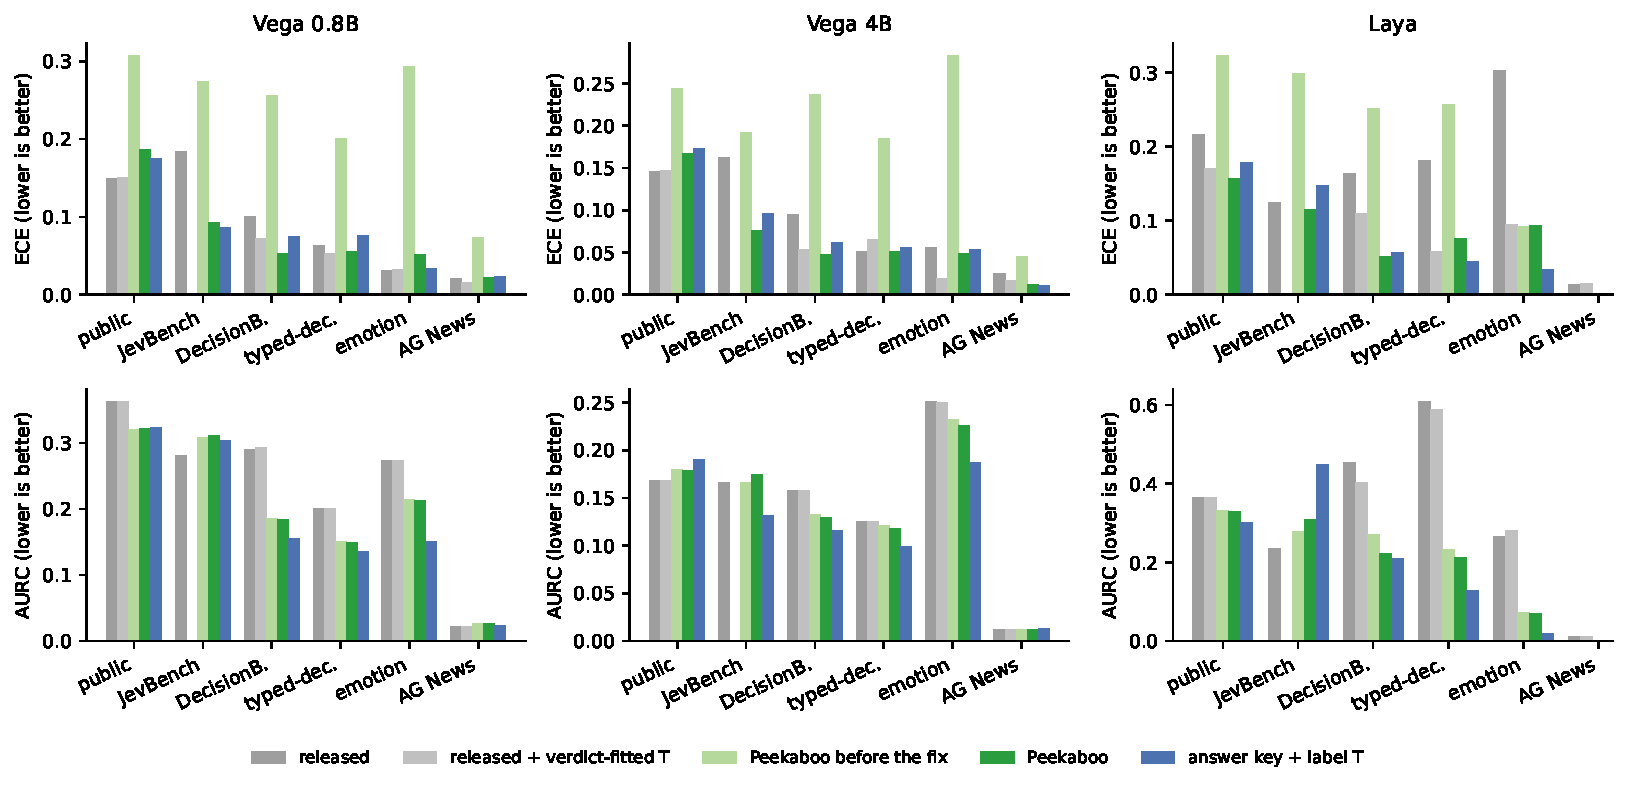
\includegraphics[width=\linewidth]{calibration.pdf}
\caption{ECE (top) and area under the risk-coverage curve (bottom), lower is better, for the released model, the released model with a temperature fitted from verdicts on its own calibration rows, \pk{} before and after the honesty fix, and the answer-key adapter with a label-fitted temperature. Laya: the encoder-unfrozen arms.}
\label{fig:cal}
\end{figure}

\begin{figure}[t]\centering
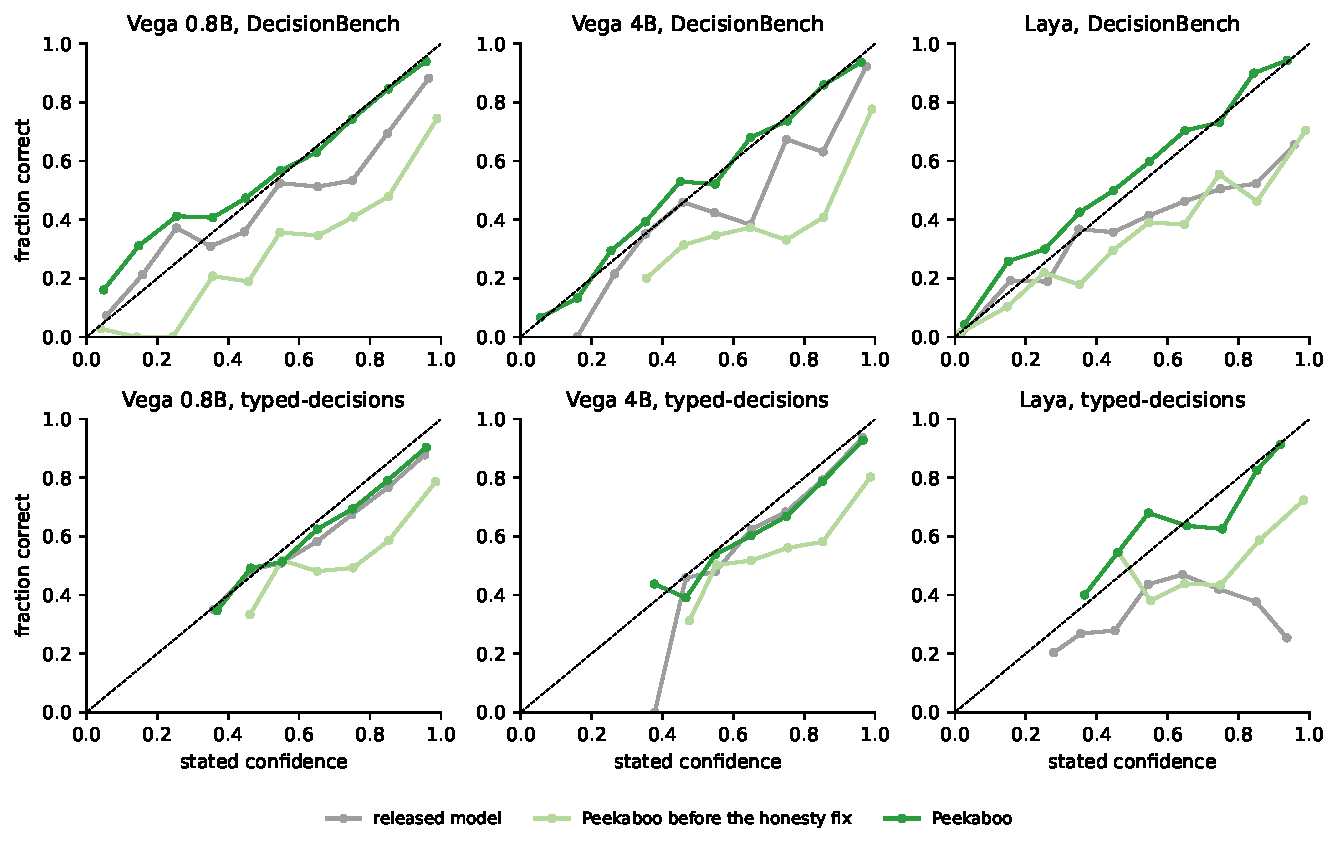
\includegraphics[width=0.9\linewidth]{reliability.pdf}
\caption{Reliability diagrams (10 bins on the confidence of the predicted option) on DecisionBench and typed-decisions: released model, \pk{} before the honesty fix, \pk{} after it (Laya: encoder unfrozen).}
\label{fig:rel}
\end{figure}

\begin{table}[tbp]\centering\scriptsize
\caption{Calibration and proper scores (lower is better; mean over seeds). ``+ T'' rows apply one temperature to the released model, fitted on its own calibration rows from verdicts on sampled answers (mean over 10 draws) or from labels.}
\label{tab:cal}
\setlength{\tabcolsep}{2.5pt}
\resizebox{\linewidth}{!}{\begin{tabular}{llrrrrrrrrrrrrrrrrrr}
\toprule
model & method & \multicolumn{3}{c}{public} & \multicolumn{3}{c}{JevBench} & \multicolumn{3}{c}{DecisionB.} & \multicolumn{3}{c}{typed-dec.} & \multicolumn{3}{c}{emotion} & \multicolumn{3}{c}{AG News} \\
 & & ECE & NLL & AURC & ECE & NLL & AURC & ECE & NLL & AURC & ECE & NLL & AURC & ECE & NLL & AURC & ECE & NLL & AURC \\
\midrule
\multicolumn{20}{l}{\textit{Vega 0.8B}} \\
 & released model & 0.150 & 1.100 & 0.363 & 0.184 & 1.262 & 0.281 & 0.101 & 1.631 & 0.291 & 0.063 & 0.753 & 0.200 & 0.031 & 1.193 & 0.274 & 0.021 & 0.291 & 0.023 \\
 & released + T from verdicts & 0.151 & 1.090 & 0.363 & -- & -- & -- & 0.072 & 1.509 & 0.294 & 0.053 & 0.747 & 0.200 & 0.033 & 1.192 & 0.274 & 0.016 & 0.289 & 0.023 \\
 & released + T from labels & 0.148 & 1.088 & 0.363 & -- & -- & -- & 0.089 & 1.515 & 0.296 & 0.050 & 0.745 & 0.201 & 0.036 & 1.191 & 0.274 & 0.016 & 0.289 & 0.023 \\
 & Peekaboo before the honesty fix & 0.308 & 2.735 & 0.321 & 0.275 & 1.758 & 0.308 & 0.257 & 3.547 & 0.186 & 0.200 & 1.354 & 0.151 & 0.293 & 3.593 & 0.215 & 0.073 & 0.707 & 0.026 \\
 & Peekaboo & 0.187 & 1.114 & 0.322 & 0.093 & 1.036 & 0.312 & 0.053 & 1.316 & 0.185 & 0.055 & 0.690 & 0.150 & 0.052 & 1.057 & 0.213 & 0.023 & 0.281 & 0.027 \\
 & Peekaboo, one pass & 0.177 & 1.102 & 0.342 & 0.079 & 1.006 & 0.287 & 0.059 & 1.376 & 0.212 & 0.059 & 0.714 & 0.160 & 0.046 & 1.045 & 0.211 & 0.012 & 0.256 & 0.020 \\
 & answer key + label temperature & 0.174 & 1.073 & 0.323 & 0.086 & 1.053 & 0.304 & 0.075 & 1.178 & 0.155 & 0.076 & 0.685 & 0.135 & 0.033 & 0.911 & 0.151 & 0.024 & 0.291 & 0.023 \\
\midrule
\multicolumn{20}{l}{\textit{Vega 4B}} \\
 & released model & 0.146 & 0.768 & 0.169 & 0.162 & 0.959 & 0.166 & 0.095 & 1.423 & 0.157 & 0.051 & 0.631 & 0.126 & 0.056 & 1.167 & 0.251 & 0.025 & 0.224 & 0.012 \\
 & released + T from verdicts & 0.147 & 0.761 & 0.169 & -- & -- & -- & 0.053 & 1.206 & 0.158 & 0.066 & 0.643 & 0.126 & 0.019 & 1.148 & 0.250 & 0.017 & 0.214 & 0.012 \\
 & released + T from labels & 0.153 & 0.764 & 0.169 & -- & -- & -- & 0.067 & 1.203 & 0.159 & 0.053 & 0.632 & 0.126 & 0.019 & 1.148 & 0.250 & 0.012 & 0.211 & 0.012 \\
 & Peekaboo before the honesty fix & 0.244 & 2.374 & 0.180 & 0.192 & 1.316 & 0.166 & 0.237 & 3.328 & 0.132 & 0.185 & 1.237 & 0.121 & 0.283 & 2.981 & 0.232 & 0.046 & 0.407 & 0.012 \\
 & Peekaboo & 0.167 & 0.836 & 0.179 & 0.076 & 0.783 & 0.174 & 0.047 & 1.095 & 0.129 & 0.051 & 0.637 & 0.118 & 0.049 & 1.087 & 0.226 & 0.012 & 0.208 & 0.012 \\
 & Peekaboo, one pass & 0.143 & 0.775 & 0.171 & 0.064 & 0.776 & 0.178 & 0.040 & 1.135 & 0.144 & 0.055 & 0.643 & 0.123 & 0.028 & 1.115 & 0.235 & 0.013 & 0.208 & 0.013 \\
 & answer key + label temperature & 0.173 & 0.840 & 0.191 & 0.096 & 0.679 & 0.131 & 0.062 & 1.051 & 0.116 & 0.056 & 0.567 & 0.100 & 0.054 & 0.996 & 0.187 & 0.011 & 0.220 & 0.013 \\
\midrule
\multicolumn{20}{l}{\textit{Laya}} \\
 & released model & 0.217 & 1.651 & 0.365 & 0.125 & 0.928 & 0.236 & 0.165 & 2.062 & 0.454 & 0.182 & 1.361 & 0.610 & 0.303 & 2.082 & 0.267 & 0.015 & 0.206 & 0.012 \\
 & released + T from verdicts & 0.171 & 1.189 & 0.365 & -- & -- & -- & 0.110 & 1.631 & 0.404 & 0.058 & 1.207 & 0.590 & 0.095 & 1.176 & 0.282 & 0.016 & 0.206 & 0.012 \\
 & released + T from labels & 0.174 & 1.159 & 0.361 & -- & -- & -- & 0.103 & 1.631 & 0.404 & 0.059 & 1.205 & 0.588 & 0.097 & 1.177 & 0.282 & 0.017 & 0.206 & 0.012 \\
 & Peekaboo, one pass & 0.163 & 1.111 & 0.364 & 0.107 & 0.911 & 0.245 & 0.075 & 1.575 & 0.389 & 0.034 & 1.194 & 0.563 & -- & -- & -- & -- & -- & -- \\
 & Peekaboo, encoder unfrozen & 0.157 & 1.088 & 0.329 & 0.115 & 1.024 & 0.309 & 0.052 & 1.392 & 0.223 & 0.077 & 0.827 & 0.213 & 0.094 & 0.665 & 0.070 & -- & -- & -- \\
 & answer-key encoder + label temperature & 0.179 & 1.025 & 0.303 & 0.148 & 1.085 & 0.448 & 0.057 & 1.296 & 0.211 & 0.045 & 0.636 & 0.129 & 0.035 & 0.313 & 0.018 & -- & -- & -- \\
\bottomrule
\end{tabular}}
\end{table}


Before the honesty fix the trained add-on is badly over-confident: ECE $\eceSmallPkRawDb$ on DecisionBench at 0.8B, $\eceBigPkRawDb$ at 4B, $\eceSmallPkRawEmo$ and $\eceBigPkRawEmo$ on emotion (Table~\ref{tab:cal}, Figure~\ref{fig:rel}). One temperature fitted from verdicts brings these to $\eceSmallPkDb$, $\eceBigPkDb$, $\eceSmallPkEmo$ and $\eceBigPkEmo$. Against the released model the picture is mixed. \pk{}'s ECE is lower on DecisionBench and JevBench at both sizes, on typed-decisions at 0.8B and on emotion and AG News at 4B, and higher on the public menu at both sizes and on emotion and AG News at 0.8B (Table~\ref{tab:cal}). The control the first version lacked, the released model with the same temperature fitted on its own calibration rows, reaches $\eceBaseTFbSmallDb$ and $\eceBaseTFbBigDb$ on DecisionBench against the released model's $\eceSmallBaseDb$ and $\eceBigBaseDb$; \pk{} is better calibrated than this control in four of the ten Vega cells where both exist (DecisionBench at both sizes, typed-decisions and AG News at 4B) and worse in the other six. Much of the ECE improvement the first version credited to the adapter is the temperature. On proper scores the adapter does help: its Brier score is below the released model's on every Vega benchmark but the public menu at 4B, and on DecisionBench at 0.8B its NLL is $\nllSmallPkDb$ against the released model's $\nllSmallBaseDb$, though above the labelled adapter's $\nllSmallSupDb$. Selective risk (AURC), which depends almost only on how rows are ranked by confidence, is better than the released model's on DecisionBench, typed-decisions and emotion at both sizes and on the public menu at 0.8B, and worse on JevBench at both sizes, on the public menu at 4B and on AG News at 0.8B (Figure~\ref{fig:cal}). The fitted temperatures range from $\Tmin$ to $\Tmax$ with a median of $\Tmedian$ (Figure~\ref{fig:switch_T}); part of each is inherited from the released model, which itself prefers a temperature above 1 on most benchmarks ($\TBaseTFbSmallDb$ on DecisionBench at 0.8B).

\subsection{The KL term and the switch}
\label{sec:ablation}

\begin{figure}[t]\centering
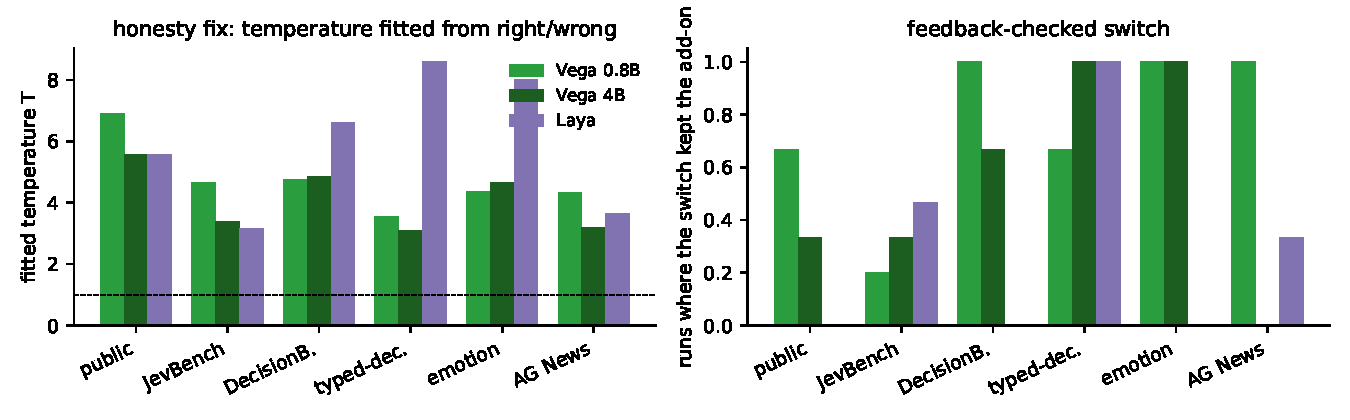
\includegraphics[width=0.9\linewidth]{switch_T.pdf}
\caption{Left: the temperature fitted from verdicts per model and benchmark (dashed line at $T = 1$; Laya: encoder unfrozen). Right: the share of runs in which the switch, comparing best answers on the calibration rows, kept the add-on; black ticks show the first version's switch on the same runs, which compared sampled answers.}
\label{fig:switch_T}
\end{figure}

Removing the KL term changes eight-pass \pk{} by $\gainSmallPkDbVsKlzero$ $\ciSmallPkDbVsKlzero$ points on DecisionBench at 0.8B and $\gainBigPkDbVsKlzero$ $\ciBigPkDbVsKlzero$ at 4B (positive means the term helps; Table~\ref{tab:h2h}), $\gainSmallPkTypedVsKlzero$ and $\gainBigPkTypedVsKlzero$ on typed-decisions, $\gainSmallPkPubVsKlzero$ and $\gainBigPkPubVsKlzero$ on the public menu, and $\gainSmallPkEmoVsKlzero$ and $\gainBigPkEmoVsKlzero$ $\ciBigPkEmoVsKlzero$ on emotion. The term is decisive in one cell, emotion at 4B, where the run without it collapsed, and that is the only KL contrast that survives Holm adjustment; elsewhere it is worth between $-0.6$ and $+2.2$ points and none of those differences survives. The no-KL arm has three seeds on DecisionBench and on JevBench at 0.8B, and one elsewhere. The first version's ``where the method lives'' was too strong.

The switch now compares best answers, which takes two verdicts on the same question, one of them on an answer the system did not serve; a deployment would have to run it as a held-out comparison on a slice of traffic. At 0.8B it turns the add-on off on JevBench, where \pk{} loses $\absSmallPkJev$ points (gain with the switch $\gainSmallPkSwJev$), and keeps it on every other benchmark. At 4B it keeps the add-on on DecisionBench and emotion; it also keeps it on the public menu, where \pk{} is $\gainBigPkPub$ (not significant), and it drops it in most JevBench folds and on typed-decisions, giving up gains of $\gainBigPkJev$ and $\gainBigPkTyped$ that were themselves not significant. The first version's switch, computed on the same runs, kept the add-on in $\swOnSampledBigPkDb$\% of the DecisionBench runs at 4B, where the new one keeps it in $\swOnBigPkDb$\%; the two statistics disagree in the direction Section~\ref{sec:switch} describes.

\subsection{Laya: head, encoder, and the matched fine-tune}
\label{sec:laya}

\begin{figure}[t]\centering
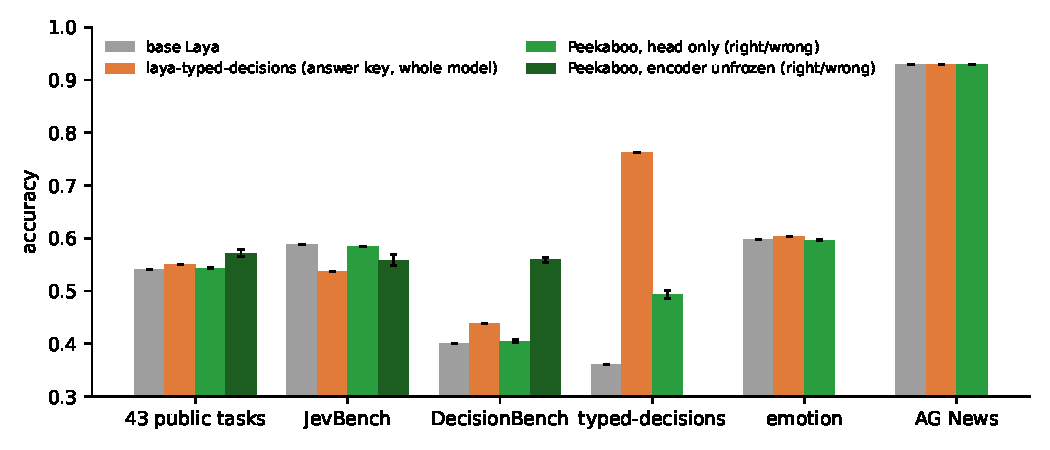
\includegraphics[width=0.85\linewidth]{laya.pdf}
\caption{Laya with the encoder unfrozen: gain over released Laya of the typed-decisions fine-tune (in-domain only on typed-decisions), the matched answer-key fine-tune (same rows, passes and KL term, early-stopped), \pk{} with eight passes and with one pass, and head-only \pk{} with one pass. Encoder arms have three seeds on the public menu and JevBench, two on DecisionBench and one on typed-decisions and emotion; AG News was not run.}
\label{fig:laya}
\end{figure}

With the encoder frozen, a trainable copy of Laya's head learns a prior shift and little else; in the first version's grid, eight passes gave $\gainVoneLayaPkTyped$ points on typed-decisions where a 71-offset prior from the same verdicts gave $\gainVonePriorFbLayaTyped$, and in this grid one pass gives $\gainLayaPkOneTyped$. With the encoder unfrozen, verdicts move the whole model: $\gainLayaPkEncTyped$ $\ciLayaPkEncTyped$ on typed-decisions with eight passes, $\gainLayaPkEncOneTyped$ with one, $\gainLayaPkEncEmo$ on emotion, $\gainLayaPkEncDb$ on DecisionBench and $\gainLayaPkEncPub$ on the public menu. The comparison the first version lacked is the same fine-tune on labels: cross-entropy, same rows, passes and KL term, encoder unfrozen. It gains $\gainLayaSupEncTyped$ on typed-decisions, $\gainLayaSupEncEmo$ on emotion, $\gainLayaSupEncDb$ on DecisionBench and $\gainLayaSupEncPub$ on the public menu; \pk{} minus this arm is $\gainLayaPkEncTypedVsSupEnc$ $\ciLayaPkEncTypedVsSupEnc$ on typed-decisions, $\gainLayaPkEncEmoVsSupEnc$ $\ciLayaPkEncEmoVsSupEnc$ on emotion, $\gainLayaPkEncDbVsSupEnc$ on DecisionBench and $\gainLayaPkEncPubVsSupEnc$ on the public menu. At matched capacity and data, labels beat eight rounds of verdicts clearly on typed-decisions and emotion. On DecisionBench and the public menu the gap is one to two points and within the noise. On JevBench the two are level: \pk{} minus the same-recipe arm is $\gainLayaPkEncJevVsSupEnc$ $\ciLayaPkEncJevVsSupEnc$ and minus the early-stopped one $\gainLayaPkEncJevVsSupEncEs$ $\ciLayaPkEncJevVsSupEncEs$. One pass costs the encoder arm a lot ($\gainLayaPkEncOneTypedVsPkEnc$ on typed-decisions, $\gainLayaPkEncOneEmoVsPkEnc$ on emotion against eight passes); no one-pass labelled encoder arm was run, so these have no matched label comparator. The head-only one-pass arm barely moves from the released model ($\gainLayaPkOneTyped$ on typed-decisions) where the one-pass labelled head gains $\gainLayaSupOneTyped$.
On typed-decisions the matched fine-tune reaches $\accLayaSupEncTyped$ against the released \texttt{laya-typed-decisions} checkpoint's $\accLayaTdTyped$, so our labelled arm is a fair stand-in for Laya's own recipe. Away from typed-decisions the released fine-tune is a transfer model that never saw the benchmark, and in-domain training of any kind beats it: \pk{} with the encoder is $\gainLayaPkEncEmoVsTd$ above it on emotion and $\gainLayaPkEncDbVsTd$ on DecisionBench, the labelled encoder arm $\gainLayaSupEncEmoVsTd$ and $\gainLayaSupEncDbVsTd$. Those numbers say that fine-tuning on a benchmark's own rows helps on that benchmark; they say nothing about verdicts against labels, and we do not use them to.

\subsection{typed-decisions without Vega's shipped adapter}
\label{sec:noship}
\begin{table}[tbp]\centering\small
\caption{typed-decisions on Vega with the shipped \texttt{typed\_decisions} adapter, which was fitted with labels on this feedback pool, switched off. Accuracy (mean over seeds) and gain over the corresponding released model.}
\label{tab:noship}
\resizebox{\linewidth}{!}{\begin{tabular}{llrrrr}
\toprule
model & method & accuracy, adapters on & gain & accuracy, adapters off & gain \\
\midrule
Vega 0.8B & released engine & 0.666 & -- & 0.377 & -- \\
Vega 0.8B & answer-key adapter (8) & 0.737 {\scriptsize$\pm$0.002} & +7.0 {\scriptsize[+5.0, +9.1]} & 0.693 {\scriptsize$\pm$0.013} & +31.6 {\scriptsize[+28.9, +34.4]} \\
Vega 0.8B & Peekaboo (8) & 0.728 {\scriptsize$\pm$0.007} & +6.2 {\scriptsize[+4.2, +8.2]} & 0.507 {\scriptsize$\pm$0.028} & +13.0 {\scriptsize[+9.8, +16.5]} \\
Vega 0.8B & Peekaboo (1) & 0.708 {\scriptsize$\pm$0.003} & +4.1 {\scriptsize[+2.2, +6.1]} & 0.498 {\scriptsize$\pm$0.007} & +12.1 {\scriptsize[+10.1, +14.2]} \\
Vega 4B & released engine & 0.729 & -- & 0.440 & -- \\
Vega 4B & answer-key adapter (8) & 0.769 {\scriptsize$\pm$0.001} & +4.0 {\scriptsize[+2.5, +5.6]} & 0.748 {\scriptsize$\pm$0.006} & +30.8 {\scriptsize[+27.8, +33.9]} \\
Vega 4B & Peekaboo (8) & 0.746 {\scriptsize$\pm$0.010} & +1.7 {\scriptsize[-0.1, +3.6]} & 0.685 {\scriptsize$\pm$0.027} & +24.6 {\scriptsize[+21.0, +28.5]} \\
Vega 4B & Peekaboo (1) & 0.749 {\scriptsize$\pm$0.004} & +2.0 {\scriptsize[+0.7, +3.5]} & 0.661 {\scriptsize$\pm$0.004} & +22.2 {\scriptsize[+19.4, +25.0]} \\
\bottomrule
\end{tabular}}
\end{table}

Vega's released \texttt{typed\_decisions} adapter was fitted on the pool our methods learn from, so on this benchmark ``released Vega'' already carries those labels. With the shipped adapters switched off the released engine scores $\accSmallNoshipBaseTyped$ at 0.8B and $\accBigNoshipBaseTyped$ at 4B (Table~\ref{tab:noship}). From that start eight-pass \pk{} gains $\gainSmallPkNoshipTypedVsNoshipBase$ $\ciSmallPkNoshipTypedVsNoshipBase$ and $\gainBigPkNoshipTypedVsNoshipBase$ $\ciBigPkNoshipTypedVsNoshipBase$, the labelled adapter $\gainSmallSupNoshipTypedVsNoshipBase$ and $\gainBigSupNoshipTypedVsNoshipBase$, and one-pass \pk{} $\gainSmallPkOneNoshipTypedVsNoshipBase$ and $\gainBigPkOneNoshipTypedVsNoshipBase$. The gap between verdicts and labels, $\gainSmallPkNoshipTypedVsSupNoship$ at 0.8B and $\gainBigPkNoshipTypedVsSupNoship$ at 4B, is far wider than with the shipped adapter on, which is the clearest demonstration in the paper of what the $\pi(y)$ weighting means: when the released model puts little probability on the gold answer, a verdict on a sampled answer rarely finds it, and labels do.
